\chapter{ODOOS ACOMPLISHMENTS REGARDING PLM AND MES ODOO 在 PLM 的成就製造執行系統} 
\pagenumbering{arabic} %設定頁號阿拉伯數字
\setcounter{page}{72}  %設定頁數

\fontsize{12}{2.5pt}\selectfont {This chapter aims to summarize the strengths and weaknesses of the Odoo software focusing on the questions raised on section 4.2. It will also comment Odoo functionalities or lack thereof noticed throughout the simulation also taking the questions into account.}\\[1pt]

\fontsize{12}{2.5pt}\selectfont {本章旨在總結 Odoo 軟體的優點和缺點重點關注4.2節提出的問題。 它還會評論 Odoo 功能或考慮到問題,整個模擬過程中也注意到缺乏這一點。}\\[15pt]

\section{How does the software deals with items? 軟體如何處理專案?}
\fontsize{12pt}{2.5pt}\selectfont
{Overall, the Odoo software presents the user with a wide variety of digital items that can be used to represent several aspects of
manufacturing as well as other aspects of business.This is mainly due to the way the Odoo ERP functionality uses items to track the pull and push actions throughout its use, that is also how automation is achieved in the software.}\\[1pt]

\fontsize{12pt}{2.5pt}\selectfont 
{總體而言,Odoo 軟體為用戶提供了各種各樣的數位項目,可以可用於表示製造的多個方面以及業務的其他方面。這主要是由於 Odoo ERP 功能使用項目來追蹤拉動和在整個使用過程中推動操作,這也是軟體實現自動化的方式。}\\[1pt]

\section{Are all aspects of the product lifecycle represented? 是否代表了產品生命週期的所有面向?}
\fontsize{12pt}{2.5pt}\selectfont 
{One of the disadvantages of being derived from a ERP system is that it focus on the primary scope of ERP (Figure 2) ,that is,
production and sales. The Items in Odoo reflect that. For instance, the development part of the life cycle during the simulation, although the representation was possible it certainly felt like a stretch of functionalities made for the production phase rather than development is self (Figure 70). When developing prototypes for instance many of the steps like creating an ECO just to carry files in the beginning and going through many steps every time an adjustment in the prototype was made felt too bureaucratic or too much of a workaround..}\\[1pt]

\fontsize{12pt}{2.5pt}\selectfont
{源自 ERP 系統的缺點之一是它專注於ERP的主要範圍(圖2),即生產和銷售。 Odoo 中的項目反映那。 例如,模擬過程中生命週期的開發部分,儘管代表性是可能的,它確實感覺像是為生產階段而不是開發階段是自我的(圖70)。 開發原型時例如,許多步驟,例如建立 ECO 只是為了在開始時攜帶文件,每次原型調整時也感覺要經歷許多步驟官僚主義或太多的解決方法。}\\[1pt]

\begin{figure}[hbt!]
\begin{center}
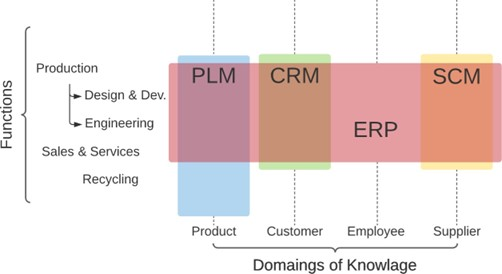
\includegraphics[width=15cm]{70}
\caption{\Large  Diagram representing Odoo scope of ERP 代表 ERP 的 Odoo 範圍的圖表}\label{fig.70}
\end{center}
\end{figure}

\section{How well are each of those items represented? 這些項目的表現如何?}
\fontsize{12pt}{2.5pt}\selectfont 
{Representation levels of the items vary depending on how the item is used. A good example of that is the material focus of product items. In the sense that everything is considered a product with very little distinction between prototypes or raw materials. The
representation of product items or BOM items is very high with a lot of metadata and useful connections to other items. However, even within the manufacturing application there are some items that lack attention. Operations for instance are items that could benefit greatly from more upload capabilities like 3D printing or CNC files. As automation is becoming more widespread in production it is no longer enough to have only PDF or slide instructions.Additionally, other items do not have the ability of holding files not even with the use ofECOs .}\\[1pt]

\fontsize{12pt}{2.5pt}\selectfont
{項目的表示等級會根據項目的使用方式而改變。 一個好的例如,產品的材質重點。 從某種意義上說,一切都是被認為是原型或原材料之間幾乎沒有區別的產品。 這產品項目或 BOM 項的表示非常高,具有大量元資料且非常有用與其他項目的連接。 然而,即使在製造應用中也存在
一些缺乏關注的項目。 例如,營運是可以受益匪淺的項目來自更多上傳功能,如 3D 列印或 CNC 檔案。 隨著自動化逐漸成為在生產中更加廣泛,僅 PDF 或幻燈片說明已不再足夠。此外,即使使用其他項目,也沒有保存文件的能力生態系統}\\[1pt]

\section{How easy it is to create a brand-new product? 創造一個全新的產品有多容易?}
\fontsize{12pt}{2.5pt}\selectfont 
{Product creation is one of the most straightforward procedures in Odoo, it really comes down to using either the Inventory
application or the Manufacturing application to create a new Product and then fill in its metadata. }\\[1pt]

\fontsize{12pt}{2.5pt}\selectfont
{產品創建是 Odoo 中最簡單的過程之一,它真的來了直至使用庫存應用程式或製造應用程式來創建新產品,然後填寫其元資料。}\\[1pt]

\section{How is the product depicted? 產品是如何描述的?}
\fontsize{12pt}{2.5pt}\selectfont 
{The product depiction is clear and concise, the product item allows for an image to be uploaded to the item and used as an icon. The ERP nature of the product items in Odoo means that the metadata is reasonably bias toward information that is used to manage storage and inventory (Weight, Volume, Quantity etc.) but the item also allows for written description as well as providing links to the BOMs and ECOs related to the product. }\\[1pt]

\fontsize{12pt}{2.5pt}\selectfont
{產品描述清晰簡潔,產品項目允許通過圖像上傳到項目並用作圖標。 Odoo 中產品項目的 ERP 性質意味著元資料合理地偏向用於管理儲存和庫存(重量、體積、數量等),但該物品也允許書面描述以及提供與產品相關的 BOM 和 ECO 的連結。}\\[1pt]

\section{How does the product integrate and reference relevant files? 產品如何整合和引用相關文件?}
\fontsize{12pt}{2.5pt}\selectfont 
{There is surely a reasonable attempt in allowing the most valuable items (Product and BOMs) to be able to manage and reference relevant files. However, Odoo does not implement much more than the bare minimum as far as file management goes. The most it can do is allow for files to be uploaded and download manually. This means that whenever someone makes a change in a file it needs to be manually uploaded in ECO. Integration with most files is inexistent except for operation items because the instruction files can be opened and interacted within Odoo during the production. }\\[1pt]

\fontsize{12pt}{2.5pt}\selectfont
{肯定有合理的嘗試來允許最有價值的物品(產品和BOM)能夠管理和引用相關文件。 然而,Odoo 並沒有實現就文件管理而言,遠遠超出了最低限度。 它最多能做的就是允許手動上傳和下載檔案。 這意味著每當有人對需要手動上傳到 ECO 的檔案進行更改。 與大多數文件集成
由於指令檔可以打開,除操作項外不存在在製作過程中與 Odoo 互動。}\\[1pt]

\section{Does changing one affects the other? 改變一個會影響另一個嗎?}
\fontsize{12pt}{2.5pt}\selectfont 
{It does not, files are mostly dealt by Odoo as paperwork for later reference. Anything added file wise that could entail a change in the product or BOM metadata will require someone to be aware of the change and update the information manually.}\\[1pt]

\fontsize{12pt}{2.5pt}\selectfont
{事實並非如此,文件大多由 Odoo 作為文書處理以供以後參考。 任何事物明智地添加文件可能需要更改產品或 BOM 元數據有人了解更改並手動更新資訊。}\\[1pt]

\section{How easy it is to create a brand-new production process? 創造全新的生產流程談何容易?}
\fontsize{12pt}{2.5pt}\selectfont 
{As mentioned before the item the best represents the process is the bill of materials. This item class requires an existing product to be associated with, other that the BOM is no harder to create than a product item.}\\[1pt]

\fontsize{12pt}{2.5pt}\selectfont
{如前所述,最能代表流程的項目是物料清單。 這項目類別需要與現有產品關聯,除此之外,BOM 並不困難建立一個產品項目。}\\[1pt]

\section{How the process is depicted? 其過程是如何描述的?}
\fontsize{12pt}{2.5pt}\selectfont 
{The process is depicted in the BOM as a list of components (other product items) and operations that are carried out in as specific order to produce a number of end products. This representation seems to sit well with the production procedure. Metadata is kept to a minimum but there is still the capability to offer a text description.}\\[1pt]

\fontsize{12pt}{2.5pt}\selectfont
{此流程在 BOM 中描述為元件清單(其他產品項目)和按特定順序進行的操作,以生產多種最終產品。 這代表性似乎與生產程序吻合。 元資料保存到最低限度,但仍能提供文字描述。}\\[1pt]

\section{How does the process integrate and reference the product itproduces? 流程如何整合並引用產品產生?}
\fontsize{12pt}{2.5pt}\selectfont 
{The integration between the BOM and the product items is by far the most well done in Odoo. Changes made in the BOM affect production and are directly linked to the product.Whenever metadata changes are possible and said aspect is represented in the product itemas well the change of one is inherited by the other.}\\[1pt]

\fontsize{12pt}{2.5pt}\selectfont
{BOM 和產品項目之間的整合是迄今為止做得最好的奧杜。 BOM 中的變更會影響生產並直接與產品相關。每當元資料可能發生變化並且所述方面在產品項中表示時一個人的改變也會被另一個人繼承。}\\[1pt]

\section{Does changing one affects the other? 改變一個會影響另一個嗎?}
\fontsize{12pt}{2.5pt}\selectfont 
{As far as inventory and manufacturing is concerned integration is and referencing is well implemented. Production results flawlessly in the resulting changes in inventory and the navigation path of the GUI is very well optimized. It does not take more than 3 or 4 clicks to get from one product to another or to navigate to other relevant items. }\\[1pt]

\fontsize{12pt}{2.5pt}\selectfont
{就庫存和製造而言,整合和參考都很好實施的。 生產結果完美地體現在庫存和生產的變化上GUI 的導航路徑得到了很好的最佳化。 點擊次數不超過 3 或 4 次從一種產品轉到另一種產品或導航至其他相關項目。}\\[1pt]

\section{How easy is to improve an existing product/ production process? 改善現有產品/生產流程有多容易?}
\fontsize{12pt}{2.5pt}\selectfont 
{As mentioned previously, all improvements in Odoo are performed using engineering change orders. These are applied to product items or bill of materials. Creating ECOs is quite easy and organized, the ECO is an item on itself that symbolizes a signal given to create change, once effective, it symbolizes an increment on the product or process.}\\[1pt]

\fontsize{12pt}{2.5pt}\selectfont
{如前所述,Odoo 中的所有改進都是使用工程來執行的更改訂單。 這些適用於產品項目或物料清單。 創建 ECO 相當重要,ECO 簡單且有條理,它本身就是一個象徵著創造的訊號變革一旦生效,就像徵著產品或流程的增量。}\\[1pt]

\section{How easy it is to update its metadata 更新元數據有多容易}
\fontsize{12pt}{2.5pt}\selectfont 
{It is easy to update any metadata regarding any item in Odoo; however, it is wise to point out that since the ECOs are separate items that are just point by products or BOMs many of the changes are not automatic and require manual intervention. I.e. an ECO will not change the text description of the product for instance. If the new update were to require a change on that description it would require a manual intervention from the user in the product item. Doing that is easy, but it is an extra task that will not be tracked by the ECO.  }\\[1pt]

\fontsize{12pt}{2.5pt}\selectfont
{更新 Odoo 中任何項目的任何元資料都很容易; 然而,明智的做法是指出指出由於 ECO 是單獨的項目,僅按產品或 BOM 點,因此許多更改不是自動的,需要手動幹預。 IE。 ECO 不會改變例如產品的文字描述。 如果新的更新需要更改根據該描述,需要使用者對產品項目進行手動幹預。這樣做很容易,但這是一項額外的任務,ECO 不會追蹤。}\\[1pt]

\section{How easy it is to determine the effects of the change? 確定變革的影響有多容易?}
\fontsize{12pt}{2.5pt}\selectfont 
{Odoo feedback of information is mainly done in a manufacturing order basis. The information available is clear and ECOs do not affect MOs that are already under way so the effects of an applied ECO would not be hard to notice. However, it is good to point out that in the way the performance information is displayed there is no indication of the product revision or the ECO applied. This means that the user would need to first figure when the ECO was applied, then navigate to the equivalent MO in the data to draw its conclusions. Although not a problem for recent changes this does becomes problematic if someone want to analyze effects of old changes.}\\[1pt]

\fontsize{12pt}{2.5pt}\selectfont
{Odoo的資訊回饋主要是在製造訂單的基礎上完成的。 這現有資訊很明確,ECO 不會影響已經在進行的 MO,因此應用 ECO 的效果不難注意到。 不過,值得指出的是性能資訊的顯示方式沒有任何產品的指示修訂或應用 ECO。 這意味著用戶需要先計算應用 ECO,然後導航到資料中的等效 MO 來得出結論。雖然最近的變化不是問題,但如果有人想要的話,這確實會成為問題分析舊變化的影響。}\\[1pt]

\section{How does the software deals with different product revisions? 軟體如何處理不同的產品版本?}
\fontsize{12pt}{2.5pt}\selectfont 
{Version control is something well covered by the 1 to N relation between product/BOM
and linked ECOs. Every product will have a tab containing all the ECOs applied to it in
chronological order effectively working as a timeline representing the item evolution.}\\[1pt]

\fontsize{12pt}{2.5pt}\selectfont
{產品/BOM 之間的 1 對 N 關係很好地涵蓋了版本控制和連結的 ECO。 每個產品都會有一個選項卡,其中包含應用於該產品的所有 ECO時間順序有效地作為代表專案演變的時間軸。}\\[1pt]

\section{How easy is to find data related to product or process? 尋找與產品或流程相關的數據有多容易?}
\fontsize{12pt}{2.5pt}\selectfont 
{Most of the data related to performance regarding production is concentrated under the reporting tab as mentioned in the previous chapter (Figure 71). }\\[1pt]

\fontsize{12pt}{2.5pt}\selectfont
{大多數與生產績效相關的數據都集中在上一章提到的報告標籤(圖 71)。}\\[1pt]

\begin{figure}[hbt!]
\begin{center}
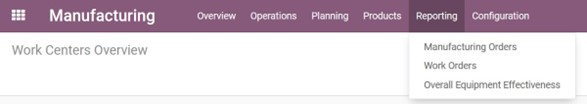
\includegraphics[width=15cm]{71}
\caption{\Large  GUI Options of data reporting 數據報告的 GUI 選項}\label{fig.71}
\end{center}
\end{figure}

\fontsize{12pt}{2.5pt}\selectfont 
{This means that as far as performance is concerned it is quite easy to find the data. The previous chapter will show examples of possible information that are available within those tabs.In addition to using this path the UI of the product item also has a tab that point to the monthly comparison of production volume regarding the product (Figure 72). Which would be more impressive if there was more than one month in the trial version of Odoo.}\\[1pt]

\fontsize{12pt}{2.5pt}\selectfont
{這意味著就效能而言,查找數據非常容易。 上一章將顯示這些標籤中可能提供的資訊的範例。除了使用此路徑之外,產品項目的 UI 還具有一個選項卡,該標籤指向有關產品的每月產量比較(圖 72)。 如果 Odoo 的試用版有超過一個月的時間,那就更令人印象深刻了。}\\[1pt]

\begin{figure}[hbt!]
\begin{center}
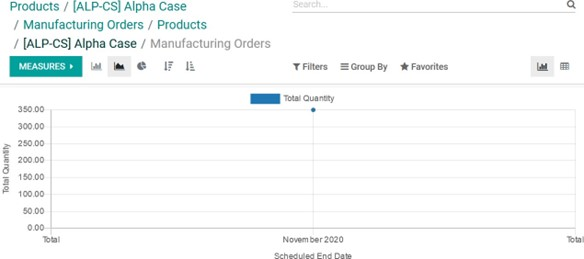
\includegraphics[width=15cm]{72}
\caption{\Large  Total quantity regarding MO from product item 產品項目中有關 MO 的總數量}\label{fig.72}
\end{center}
\end{figure}

\section{How easy is find production numbers? 要找出生產編號有多容易?}
\fontsize{12pt}{2.5pt}\selectfont 
{In addition to the previously mentioned ways, Odoo also makes available a unit forecast graph that records the ins and outs of the inventory. This is particularly useful to estimate sales and balance storage with demand (Figure 73). This feature is not mentioned to much in this work because supply and demand is not so much a MES functionality, but it is to useful to have an overview of the production.}\\[1pt]

\fontsize{12pt}{2.5pt}\selectfont
{除了前面提到的方法之外,Odoo 還提供了一個單位預測圖,記錄庫存的來龍去脈。 這對於估計銷售量以及平衡儲存與需求特別有用(圖 73)。 此功能在本工作中並未過多提及,因為供應和需求與其說是 MES 功能,但它對於了解生產情況非常有用。}\\[1pt]

\begin{figure}[hbt!]
\begin{center}
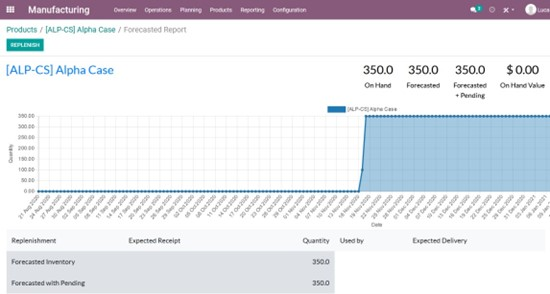
\includegraphics[width=15cm]{73}
\caption{\Large  Unit forecast overview 單位預測概覽}\label{fig.73}
\end{center}
\end{figure}

\section{How does Odoo generate performance data? Odoo 如何產生效能數據?}
\fontsize{12pt}{2.5pt}\selectfont 
{The astute reader will notice that all the data mentioned so far is derived from the time to completion of the operations been carried out, the related amount to the MO and the workcenter utilized. Even so it is impressive how much information can be drawn especially considering that it is all generated automatically.}\\[1pt]

\fontsize{12pt}{2.5pt}\selectfont
{精明的讀者會注意到,到目前為止提到的所有數據都是從完成作業的時間、與 MO 和所使用的工作中心相關的數量得出的。 即便如此,可以提取的資訊量仍然令人印象深刻,特別是考慮到這些資訊都是自動產生的。}\\[1pt]

\section{How does the software present performance change as a result of a upgrade? 升級後軟體的效能有何變化?}
\fontsize{12pt}{2.5pt}\selectfont 
{In order to identify the change, the user must identify the MOs following the change and see the difference based on that. Ideally it would be nice if the graphical information showed the revision of the product, but this is not present as of Odoo V13.}\\[1pt]

\fontsize{12pt}{2.5pt}\selectfont
{為了識別更改,使用者必須識別更改後的 MO,並基於此查看差異。 理想情況下,如果圖形資訊顯示產品的修訂版本就好了,但從 Odoo V13 開始不存在這種情況。}\\[1pt]

\chapter{CONCLUSION 結論} 

\fontsize{12pt}{2.5pt}\selectfont 
{In chapter 2 I referenced a diagram that represents a theoretical ideal of how the integration of PLM with other systems should be (Figure 74). In that diagram the reader can notice that ideally PLM would be the center of the system with other systems (Including ERP) attached to it. Different from said diagram the Odoo software takes ERP as the center with other systems attached to it. This work has shown that it is certainly possible to use Odoo for PLM and MES however it has also shown that the PLM and MES implementation presents some weaknesses.}\\[1pt]

\fontsize{12pt}{2.5pt}\selectfont
{在第 2 章中,我引用了一個圖表,它代表了 PLM 與其他系統整合的理論理想(圖 74)。 在該圖中,讀者可以注意到,理想情況下,PLM 將成為系統的中心,並附上其他系統(包括 ERP)。 與上述圖表不同的是,Odoo 軟體以 ERP 為中心,其他系統依附於此。 這項工作表明,當然可以將 Odoo 用於 PLM 和 MES,但它也表明 PLM 和 MES 的實施存在一些弱點。}\\[1pt]

\begin{figure}[hbt!]
\begin{center}
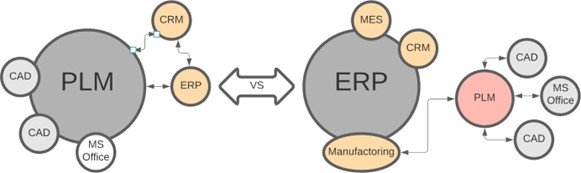
\includegraphics[width=15cm]{74}
\caption{\Large  Comparison to the left the adapted diagram as theorized by Saaksvuori, A. and Immonen, A. (2008), to the right Odoo take on how systems interact. 與左側 Saaksvuori, A. 和 Immonen, A. (2008) 理論化的改編圖相比,右側 Odoo 展示了系統如何交互作用。}\label{fig.74}
\end{center}
\end{figure}

\fontsize{12pt}{2.5pt}\selectfont 
{The lack of file upload support on things like operation items, work centers or equipment is something of some concern especially considering 3D printing or CNC because access to the CAD files would prove helpful to the operators. Also, there is a gap in between the facets of product and tool when the company is taking upon themselves to develop and produce said tooling (similar situation founded when developing the molds in the simulation).}\\[1pt]

\fontsize{12pt}{2.5pt}\selectfont
{操作項目、工作中心或裝置等缺乏文件上傳支援是一個令人擔憂的問題,特別是考慮到 3D 列印或 CNC,因為存取 CAD 檔案對操作員很有幫助。 此外,當公司自行開發和生產所述工具時,產品和工具之間存在差距(在模擬中開發模具時也會出現類似情況)。}\\[1pt]

\fontsize{12pt}{2.5pt}\selectfont 
{In addition, although MES provide detailed graphical representation regarding the dataset that it has, it is limited to data derived from the time to completion of the operations been carried out. For instance, it would be very valuable if graphical representation regarding quality control was easily available as well.}\\[1pt]

\fontsize{12pt}{2.5pt}\selectfont
{此外,雖然 MES 提供了有關其擁有的資料集的詳細圖形表示,但它僅限於從已執行操作完成的時間得出的資料。 例如,如果品質控制的圖形表示也很容易獲得,那將非常有價值。}\\[1pt]

\fontsize{12pt}{2.5pt}\selectfont 
{All that said, applying ECOs to BOMs in Odoo is a procedure deserving of praise. The ECO holds the information until it is ready to be applied and then it updates the BOM automatically once the ECO is validated by responsible personnel. It might not look like something so important now because this simulation is dealing with very simple products, but it becomes exponentially more important as complexity increases. E.g. A car with thousands of parts and hundreds of nested BOMs would be considered a nightmare to control and keep track of change if a system like this was not present.}\\[1pt]

\fontsize{12pt}{2.5pt}\selectfont
{儘管如此,在 Odoo 中將 ECO 應用到 BOM 是一個值得讚揚的過程。 ECO 會保留資訊直到準備好應用,然後在負責人員驗證 ECO 後自動更新 BOM。 現在它可能看起來不那麼重要,因為這個模擬處理的是非常簡單的產品,但隨著複雜性的增加,它變得更加重要。 例如。 如果沒有這樣的系統,一輛擁有數千個零件和數百個嵌套 BOM 的汽車將被視為控制和追蹤變更的噩夢。}\\[1pt]

\fontsize{12pt}{2.5pt}\selectfont 
{This software is not perfect for PLM or MES implementation, but it does hold value in the sense of availability and integration with other systems. The functionality is there specially regarding product and process and the software has an extremely interesting integration with its natural ERP functionalities. All this makes up for a system that would suit better:}\\[1pt]

\fontsize{12pt}{2.5pt}\selectfont
{該軟體對於 PLM 或 MES 實施來說並不完美,但在可用性和與其他系統的整合方面確實具有價值。 該功能專門針對產品和流程,並且該軟體與其自然的 ERP 功能進行了非常有趣的整合。 所有這些都彌補了一個更適合的系統:}\\[1pt]

\fontsize{12pt}{2.5pt}\selectfont 
{Small business that could use PLM and MES in a smaller scale.
Companies that deal with less manufacturing and more assembly or distribution taking advantage of the All in One nature of the software.}\\[1pt]

\fontsize{12pt}{2.5pt}\selectfont
{可以在較小規模內使用 PLM 和 MES 的小型企業。
利用軟體的多合一特性,處理更少的製造和更多的組裝或分銷的公司。}\\[1pt]

\fontsize{12pt}{2.5pt}\selectfont 
{It is important to mention that the limitations of Odoo are not in the complexity of the product itself but in the complexity of the operations that surround its development. All things considered you could track a large and complex assembly if it includes only simple manufacturing operations or if more complex engineering tasks are done by suppliers. I.e. you could track the assembly of a motorcycle with ease in Odoo, but the PLM features are not polish enough to track the full evolution/development of its powertrain. It is certainly possible to do so but it would take too much time and effort from the engineering team to be considered worth it just for the sake of having an all in one solution with ERP features.}\\[1pt]

\fontsize{12pt}{2.5pt}\selectfont
{值得一提的是,Odoo 的限制不在於產品本身的複雜性,而是圍繞其開發的操作的複雜性。 考慮到所有因素,如果大型且複雜的組裝僅包括簡單的製造操作,或者如果供應商完成了更複雜的工程任務,那麼您可以追蹤大型且複雜的組裝。 IE。 您可以在 Odoo 中輕鬆追蹤摩托車的組裝,但 PLM 功能還不夠完善,無法追蹤其動力系統的完整演變/開發。 這樣做當然是可能的,但僅僅為了擁有一個具有 ERP 功能的一體化解決方案,工程團隊就會花費太多的時間和精力,才被認為是值得的。}\\[1pt]
